 \documentclass[11pt,a4paper]{article}
\usepackage[utf8]{inputenc}		% LaTeX, comprend les accents !
\usepackage[T1]{fontenc}
\usepackage{natbib}	
%\usepackage[square,sort&compress,sectionbib]{natbib}		% Doit être chargé avant babel      
\usepackage[frenchb,english]{babel}
\usepackage{lmodern}
\usepackage{amsmath,amssymb, amsthm}
\usepackage{a4wide}
\usepackage[capposition=top]{floatrow}
\usepackage{verbatim}
\usepackage{float}
\usepackage{placeins}
\usepackage{flafter}
\usepackage{longtable}
\usepackage{import}
\usepackage{pdflscape}
\usepackage{rotating}
\usepackage{hhline}
\usepackage{multirow}
\usepackage{booktabs}
\usepackage[pdftex,pdfborder={0 0 0},colorlinks=true,linkcolor=blue,urlcolor=blue,citecolor=blue,bookmarksopen=true]{hyperref}
\usepackage{eurosym}
%\usepackage{breakcites}
\usepackage[autostyle]{csquotes}
%\usepackage{datetime}
\usepackage{natbib}
\usepackage{setspace}
\usepackage{lscape}
\usepackage[usenames]{color}
\usepackage{indentfirst}
\usepackage{url}
\usepackage{enumitem}
\usepackage{multirow}
\usepackage{subcaption}
\usepackage[justification=centering]{caption}
\bibliographystyle{agsm}
\usepackage{supertabular} 
\usepackage{array}
\usepackage{longtable}
\newcommand{\isEmbedded}{true}

\graphicspath{{Figures/}}


\begin{document}

\selectlanguage{frenchb}
\title{Le corps : bon niveau de la modélisation ?}


\author{}


\maketitle

\section{Effectifs par corps en 2012.}


\section{Transitions intra-corps entre 2012 et 2013.}


On veut savoir si les transitions de carrières se font majoritairement à l'intérieur des corps, et si ces caractéristiques des transitions de carrières concernent tous les corps de façon égale.


\subsection{Echantillon des individus qui ont leur code cir renseigné en 2012 et en 2013.}

\begin{figure}[H] 
	\caption{Parts des agents restant dans un même corps entre 2012 et 2013, par corps en 2012.}
	\label{transit1} 
	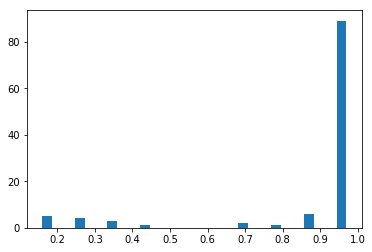
\includegraphics[scale = 0.7]{transitions_intra_corps_2012_2013_c_cir.png} 
	\begin{minipage}{15cm}
		\footnotesize
		\textsc{Population:} Individus qui ont leur code grade CIR renseigné pour les deux années 2012 et 2013 (1 640 850 identifiants contre 2 058 445 au total). 1 308 996 agents restent dans un même corps entre 2012 et 2013. 112 corps sont représentés.\\
		\textsc{Lecture:} Dans environ 85 corps sur 112, environ 100 \% des personnes qui étaient dans un de ces corps en 2012 restent dans ce même corps en 2013. \\
		\textsc{Note:} Voir les tableaux ci-dessous pour les noms des corps qui ont les plus faibles taux de rétentions et les plus forts taux de rétentions.
	\end{minipage}
\end{figure}

\begin{table}[h!]
	\label{means}
	\centering
	\caption{Description des 10 corps ayant les plus faibles taux de rétention} 
\begin{tabular}{llrrr}
	\toprule
	{} &                                     corps 2012 &  n retenus &  n corps 2012 &  part retention \\
\midrule
770  &                 Ergotherapeutes surveillants chefs &                8 &                                           62 &                                             12.90\% \\
1140 &                  Puericultrices surveillants chefs &              107 &                                          536 &                                             19.96\% \\
1091 &            Preparateur en pharmacie cadre de sante &               35 &                                          171 &                                             20.47\% \\
692  &                    Dieteticiens surveillants chefs &               15 &                                           73 &                                             20.55\% \\
1258 &      Techniciens de laboratoire surveillants chefs &               74 &                                          356 &                                             20.79\% \\
1123 &                Psychomotriciens surveillants chefs &                4 &                                           18 &                                             22.22\% \\
998  &  Manipulateurs electroradiologie surveillants c... &              131 &                                          498 &                                             26.31\% \\
825  &  Infirmiers anesthesistes reanimation surveilla... &              125 &                                          444 &                                             28.15\% \\
838  &  Infirmiers de salle d operation surveillants c... &              118 &                                          400 &                                             29.50\% \\
1008 &      Masseurs kinesitherapeutes surveillants chefs &               62 &                                          190 &                                             32.63\% \\
	     & Total des 10 corps & 679 & 2748\\
\bottomrule
\end{tabular}
\begin{minipage}{15cm}
\footnotesize
\textsc{Lecture:} 8 agents parmi 62 présents dans le corps des Ergotherapeutes surveillants chefs en 2012 restent dans ce corps en 2013 (soit 12.9 \% d'agents présents dans ce corps en 2012 toujours présents en 2013.)
\end{minipage}
\end{table}

\begin{table}[h!]
	\label{means}
	\centering
	\caption{Description des 10 corps ayant les plus forts taux de rétention} 
\begin{tabular}{llrrr}
	\toprule
	{} &                         corps 2012 &  n retenus &  n corps 2012 &  part retention \\
	\midrule
	1205 &                         Sages femmes territoriales &              488 &                                          490 &                                             99.59\% \\
	1116 &                                       Psychologues &             3592 &                                         3604 &                                             99.67\% \\
	1226 &          Sapeurs pompiers professionnels officiers &             2427 &                                         2435 &                                             99.67\% \\
	1202 &                                       Sages femmes &             9127 &                                         9156 &                                             99.68\% \\
	1094 &                          Preparateurs en pharmacie &              808 &                                          810 &                                             99.75\% \\
	696  &                 Directeurs d ecole de sages femmes &               15 &                                           15 &                                            100.00\% \\
	1069 &                               Pedicures podologues &                4 &                                            4 &                                            100.00\% \\
	1248 &                             Technicien paramedical &                1 &                                            1 &                                            100.00\% \\
	1039 &                                     Orthophonistes &              157 &                                          157 &                                            100.00\% \\
	762  &                                  Emplois nationaux &               34 &                                           34 &                                            100.00\% \\
	     & Total des 10 corps & 16 653 & 16 706\\
	\bottomrule
\end{tabular}
\begin{minipage}{15cm}
	\footnotesize
	\textsc{Lecture:} 157 agents parmi les 157 présents dans le corps des Orthophonistes en 2012 restent dans ce corps en 2013 (soit 100 \% d'agents présents dans ce corps en 2012 toujours présents en 2013.)
\end{minipage}
\end{table}

\clearpage

\begin{figure}[H] 
	\caption{Parts des agents changeant de c cir entre 2012 et 2013 et restant dans un même corps entre 2012 et 2013, par corps en 2012.}
	\label{transit1} 
	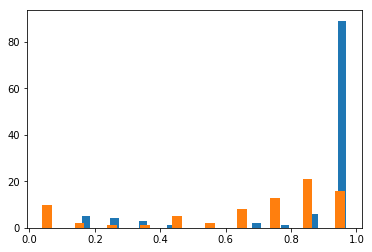
\includegraphics[scale = 0.7]{transitions_intra_corps_only_w_c_cir_change_2012_2013.png} 
	\begin{minipage}{15cm}
		\footnotesize
		\textsc{Population:} Individus qui ont leur code grade CIR renseigné pour les deux années 2012 et 2013 (1 640 850 identifiants contre 2 058 445 au total). 200 350 agents changent de grade entre 2012 et 2013. Seulement 93 976 agents ayant changé de grade restent dans un même corps entre 2012 et 2013. 79 corps sont représentés car les 112 - 79 autres n'ont pas d'agents changeant de grade entre 2012 et 2013.\\
		\textsc{Lecture:} Dans 21 corps sur 79 corps pour lesquels des agents changent de grades entre 2012 et 2013, environ 90 \% des personnes qui étaient dans un de ces corps en 2012 restent dans ce même corps en 2013. \\
		\textsc{Note:} Voir les tableaux ci-dessous pour les noms des corps qui ont les plus faibles taux de rétentions et les plus forts taux de rétentions d'agents qui changent de grades.
	\end{minipage}
\end{figure}

\begin{table}[h!]
	\label{means}
	\centering
	\caption{Description des 10 corps ayant les plus faibles taux de rétention d'agents changeant de grades} 
	\begin{tabular}{llrrr}
	\toprule
	{} &                                     corps 2012 &  n retenus &  n corps 2012 &  part retention \\
	\midrule
	819  &  Infirmiers de salle d operation surveillants c... &                1 &                                          283 &                                              0.35\% \\
	889  &                      Infirmiers surveillants chefs &               39 &                                         7797 &                                              0.50\% \\
	978  &  Manipulateurs electroradiologie surveillants c... &                2 &                                          369 &                                              0.54\% \\
	1042 &                            Ouvriers professionnels &               10 &                                         1198 &                                              0.83\% \\
	1112 &                  Puericultrices surveillants chefs &                4 &                                          433 &                                              0.92\% \\
	806  &  Infirmiers anesthesistes reanimation surveilla... &                3 &                                          322 &                                              0.93\% \\
	1063 &                            Personnels de direction &                2 &                                           81 &                                              2.47\% \\
	108  &                   Adjoints des cadres hospitaliers &                2 &                                           28 &                                              7.14\% \\
	640  &  Conseillers territoriaux des activites physiqu... &                7 &                                           98 &                                              7.14\% \\
	910  &                            Infirmiers territoriaux &              153 &                                         2003 &                                              7.64\% \\
	    & Total des 10 corps & 223 & 12 612 \\
\end{tabular}
\begin{minipage}{15cm}
\footnotesize
\textsc{Lecture:} 157 agents parmi les 157 présents dans le corps des Orthophonistes en 2012 restent dans ce corps en 2013 (soit 100 \% d'agents présents dans ce corps en 2012 toujours présents en 2013.)
\end{minipage}
\end{table}

\begin{table}[h!]
	\label{means}
	\centering
	\caption{Description des 10 corps ayant les plus forts taux de rétention d'agents changeant de grades} 
\begin{tabular}{llrrr}
	\toprule
	{} &                                     corps 2012 &  n retenus &  n corps 2012 &  part retention \\
	\midrule
	1192 &  Sapeurs pompiers professionnels non officiers &             1017 &                                         1094 &                                             92.96\% \\
	1067 &                      Preparateurs en pharmacie &               27 &                                           29 &                                             93.10\% \\
	1222 &                     Techniciens de laboratoire &              114 &                                          122 &                                             93.44\% \\
	1174 &                                   Sages femmes &              421 &                                          450 &                                             93.56\% \\
	724  &      Educateurs territoriaux de jeunes enfants &             1695 &                                         1800 &                                             94.17\% \\
	619  &          Chefs de service de police municipale &              198 &                                          210 &                                             94.29\% \\
	684  &            Directeurs des ecoles paramedicales &               19 &                                           20 &                                             95.00\% \\
	1198 &      Sapeurs pompiers professionnels officiers &              175 &                                          183 &                                             95.63\% \\
	1177 &                     Sages femmes territoriales &               51 &                                           53 &                                             96.23\% \\
	1015 &                                 Orthophonistes &                3 &                                            3 &                                            100.00\% \\
	& Total des 10 corps & 3 720 & 3 964 \\
	\bottomrule
\end{tabular}
\begin{minipage}{15cm}
\footnotesize
\textsc{Lecture:} 157 agents parmi les 157 présents dans le corps des Orthophonistes en 2012 restent dans ce corps en 2013 (soit 100 \% d'agents présents dans ce corps en 2012 toujours présents en 2013.)
\end{minipage}
\end{table}

\begin{tabular}{llrrrrrrl}
	\toprule
	{} &                                Label corps en 2012 &  Nombre agents &  Part du total &  Part cumulee du total &  taux de retention &  taux de retention si chgmt grade &  max taux de transition vers autre corps &             autre corps ac. max taux de transition \\
	\midrule
	0   &                      Agents technique territoriaux &         336163 &            0.2 &                    0.2 &              1e+00 &                               0.8 &                                     0.01 &                    Agents de maitrise territoriaux \\
	1   &                                    Aides soignants &         178694 &            0.1 &                    0.3 &              1e+00 &                               0.8 &                                    0.006 &        Infirmiers en soins generaux et specialises \\
	2   &               Adjoints administratifs territoriaux &         146233 &           0.09 &                    0.4 &              1e+00 &                               0.8 &                                     0.01 &                            Redacteurs territoriaux \\
	3   &        Infirmiers en soins generaux et specialises &         105737 &           0.06 &                    0.5 &              1e+00 &                               nan &                                    0.004 &                                         Infirmiers \\
	4   &                                         Infirmiers &          77216 &           0.05 &                    0.5 &              1e+00 &                               0.6 &                                    0.008 &        Infirmiers en soins generaux et specialises \\
	5   &         Agents des services hospitaliers qualifies &          60046 &           0.04 &                    0.6 &              1e+00 &                               nan &                                     0.03 &                                    Aides soignants \\
	6   &                            Redacteurs territoriaux &          38296 &           0.02 &                    0.6 &              1e+00 &                               0.8 &                                     0.02 &                              Attaches territoriaux \\
	7   &                    Agents de maitrise territoriaux &          36755 &           0.02 &                    0.6 &              1e+00 &                               0.7 &                                     0.02 &                           Techniciens territoriaux \\
	8   &               Adjoints administratifs hospitaliers &          34874 &           0.02 &                    0.6 &              1e+00 &                               0.8 &                                    0.003 &                               Secretaires medicaux \\
	9   &                               Adjoints d animation &          31414 &           0.02 &                    0.6 &              1e+00 &                               0.6 &                                     0.01 &               Adjoints administratifs territoriaux \\
	10  &                              Attaches territoriaux &          28216 &           0.02 &                    0.7 &              1e+00 &                               0.8 &                                    0.008 &                               Emplois fonctionnels \\
	11  &  Agents territoriaux specialises des ecoles mat... &          26325 &           0.02 &                    0.7 &              1e+00 &                               0.9 &                                    0.005 &               Adjoints administratifs territoriaux \\
	12  &                           Techniciens territoriaux &          23187 &           0.01 &                    0.7 &              1e+00 &                               0.8 &                                     0.02 &                                         Ingenieurs \\
	13  &                            Ouvriers professionnels &          21194 &           0.01 &                    0.7 &                0.9 &                             0.008 &                                     0.04 &                                   Maitres Ouvriers \\
	14  &          Assistants territoriaux sociaux educatifs &          20310 &           0.01 &                    0.7 &              1e+00 &                               0.9 &                                    0.003 &         Conseillers territoriaux sociaux educatifs \\
	15  &      Sapeurs pompiers professionnels non officiers &          17709 &           0.01 &                    0.7 &              1e+00 &                               0.9 &                                    0.003 &     Lieutenants de sapeurs pompiers professionnels \\
	16  &           Auxiliaires de puericulture territoriaux &          17113 &           0.01 &                    0.7 &              1e+00 &                               0.9 &                                    0.006 &               Adjoints administratifs territoriaux \\
	17  &                        Agents de police municipale &          14914 &          0.009 &                    0.7 &              1e+00 &                               0.9 &                                    0.003 &              Chefs de service de police municipale \\
	18  &                        Agents sociaux territoriaux &          13513 &          0.008 &                    0.7 &              1e+00 &                               0.6 &                                    0.007 &                  Auxiliaires de soins territoriaux \\
	19  &                                         Ingenieurs &          13366 &          0.008 &                    0.8 &              1e+00 &                               0.8 &                                     0.02 &                            Ingenieurs territoriaux \\
	20  &                  Agents territoriaux du patrimoine &          12210 &          0.007 &                    0.8 &              1e+00 &                               0.8 &                                    0.006 &  Assistants de conservation du patrimoine et bi... \\
	21  &                                 Agents d entretien &          11989 &          0.007 &                    0.8 &                0.9 &                               nan &                                     0.06 &                            Ouvriers professionnels \\
	22  &                      Infirmiers surveillants chefs &          11893 &          0.007 &                    0.8 &                0.3 &                             0.005 &                                      0.7 &                                     Cadre de sante \\
	23  &                                   Maitres Ouvriers &          11780 &          0.007 &                    0.8 &              1e+00 &                               0.7 &                                    0.009 &                                      Contremaitres \\
	24  &                                       Sages femmes &           9397 &          0.006 &                    0.8 &              1e+00 &                               0.9 &                                    0.001 &                         Sages femmes territoriales \\
	25  &                  Auxiliaires de soins territoriaux &           7434 &          0.005 &                    0.8 &              1e+00 &                               0.9 &                                    0.004 &               Adjoints administratifs territoriaux \\
	26  &  Educateur territoriaux des activites physiques... &           7343 &          0.004 &                    0.8 &              1e+00 &                               0.9 &                                    0.004 &                            Redacteurs territoriaux \\
	27  &          Educateurs territoriaux de jeunes enfants &           6781 &          0.004 &                    0.8 &              1e+00 &                               0.9 &                                    0.004 &          Assistants territoriaux sociaux educatifs \\
	28  &                            Animateurs territoriaux &           6390 &          0.004 &                    0.8 &              1e+00 &                               0.8 &                                     0.02 &                            Redacteurs territoriaux \\
	29  &                         Assistants socio educatifs &           5753 &          0.004 &                    0.8 &              1e+00 &                               nan &                                    0.008 &                                     Cadre de sante \\
	30  &                       Puericultrices territoriales &           4223 &          0.003 &                    0.8 &              1e+00 &                               0.9 &                                    0.004 &                              Attaches territoriaux \\
	31  &                                       Psychologues &           3680 &          0.002 &                    0.8 &              1e+00 &                               0.9 &                                   0.0008 &                                    Aides soignants \\
	32  &  Assistants de conservation du patrimoine et bi... &           3605 &          0.002 &                    0.8 &              1e+00 &                               0.9 &                                    0.004 &                       Bibliothecaires territoriaux \\
	33  &                                      Contremaitres &           3508 &          0.002 &                    0.8 &              1e+00 &                               0.7 &                                     0.01 &                                   Maitres Ouvriers \\
	34  &                            Infirmiers territoriaux &           3449 &          0.002 &                    0.8 &                0.3 &                              0.08 &                                      0.6 &                        Infirmier en soins generaux \\
	35  &   Infirmiers specialises en anesthesie reanimation &           3218 &          0.002 &                    0.8 &              1e+00 &                               0.8 &                                    0.002 &                                     Cadre de sante \\
	36  &                                     Puericultrices &           3060 &          0.002 &                    0.8 &              1e+00 &                               0.5 &                                     0.01 &                       Puericultrices territoriales \\
	37  &  Professeurs territoriaux d enseignement artist... &           2777 &          0.002 &                    0.8 &              1e+00 &                               0.9 &                                    0.003 &  Directeurs d etablissements d enseignement art... \\
	38  &                           Conducteurs ambulanciers &           2774 &          0.002 &                    0.8 &              1e+00 &                               0.8 &                                    0.005 &                                    Aides soignants \\
	39  &                               Secretaires medicaux &           2570 &          0.002 &                    0.8 &              1e+00 &                               0.7 &                                     0.01 &                                    Aides soignants \\
	40  &          Sapeurs pompiers professionnels officiers &           2521 &          0.002 &                    0.8 &              1e+00 &                             1e+00 &                                    0.002 &                        Infirmier en soins generaux \\
	41  &                               Moniteurs educateurs &           2426 &          0.001 &                    0.8 &              1e+00 &                               nan &                                     0.02 &                         Assistants socio educatifs \\
	42  &                               Emplois fonctionnels &           2282 &          0.001 &                    0.8 &                0.9 &                               0.2 &                                     0.05 &                              Attaches territoriaux \\
	43  &     Lieutenants de sapeurs pompiers professionnels &           2187 &          0.001 &                    0.8 &              1e+00 &                               0.8 &                                     0.05 &          Sapeurs pompiers professionnels officiers \\
	44  &                    Infirmiers de salle d operation &           2075 &          0.001 &                    0.8 &              1e+00 &                               0.8 &                                    0.003 &                                     Cadre de sante \\
	45  &           Manipulateurs electroradiologie medicale &           2073 &          0.001 &                    0.8 &              1e+00 &                               0.9 &                                    0.003 &  Manipulateurs electroradiologie surveillants c... \\
	46  &                         Techniciens de laboratoire &           1807 &          0.001 &                    0.8 &              1e+00 &                               0.9 &                                    0.002 &      Techniciens de laboratoire surveillants chefs \\
	47  &         Conseillers territoriaux sociaux educatifs &           1797 &          0.001 &                    0.8 &                0.9 &                               nan &                                     0.04 &                              Attaches territoriaux \\
	48  &                            Ingenieurs hospitaliers &           1697 &          0.001 &                    0.8 &              1e+00 &                               0.9 &                                    0.002 &                                         Ingenieurs \\
	49  &  Assistants territoriaux d enseignement artistique &           1380 &         0.0008 &                    0.8 &              1e+00 &                               nan &                                    0.007 &  Professeurs territoriaux d enseignement artist... \\
	50  &                              Medecins territoriaux &           1273 &         0.0008 &                    0.8 &                0.9 &                               0.6 &                                     0.06 &  Agents territoriaux specialises des ecoles mat... \\
	51  &                       Bibliothecaires territoriaux &           1204 &         0.0007 &                    0.8 &              1e+00 &                               nan &                                    0.006 &                              Attaches territoriaux \\
	52  &                                    Chefs de bureau &           1135 &         0.0007 &                    0.8 &              1e+00 &                               0.7 &                                    0.005 &                              Attaches territoriaux \\
	53  &                            Animateurs hospitaliers &           1128 &         0.0007 &                    0.8 &              1e+00 &                               nan &                                    0.004 &                            Animateurs territoriaux \\
	54  &                       Educateurs de jeunes enfants &           1112 &         0.0007 &                    0.8 &              1e+00 &                               0.9 &                                    0.006 &          Educateurs territoriaux de jeunes enfants \\
	55  &   Assistants territoriaux qualifies de laboratoire &           1084 &         0.0007 &                    0.8 &                nan &                               nan &                                      0.9 &                             Technicien paramedical \\
	56  &                   Adjoints des cadres hospitaliers &           1057 &         0.0006 &                    0.8 &              1e+00 &                              0.07 &                                     0.02 &                                    Chefs de bureau \\
	57  &                            Ingenieurs territoriaux &           1010 &         0.0006 &                    0.8 &              1e+00 &                               0.7 &                                     0.01 &                               Emplois fonctionnels \\
	58  &   Attaches territoriaux de conservation patrimoine &           1002 &         0.0006 &                    0.9 &              1e+00 &                               nan &                                    0.006 &                              Attaches territoriaux \\
	59  &                           Psychologue territoriaux &            968 &         0.0006 &                    0.9 &              1e+00 &                               0.8 &                                    0.004 &                                       Psychologues \\
	60  &              Chefs de service de police municipale &            962 &         0.0006 &                    0.9 &              1e+00 &                               0.9 &                                    0.006 &                        Agents de police municipale \\
	61  &                          Preparateurs en pharmacie &            878 &         0.0005 &                    0.9 &              1e+00 &                               0.9 &                                    0.001 &                                         Infirmiers \\
	62  &  Operateurs territoriaux des activites physique... &            848 &         0.0005 &                    0.9 &              1e+00 &                               0.8 &                                     0.03 &  Educateur territoriaux des activites physiques... \\
	63  &                         Masseurs kinesitherapeutes &            839 &         0.0005 &                    0.9 &              1e+00 &                               0.8 &                                    0.001 &               Adjoints administratifs territoriaux \\
	64  &                      Directeur general sur contrat &            825 &         0.0005 &                    0.9 &              1e+00 &                               nan &                                    0.005 &         Personnel direction etablissements sociaux \\
	65  &                              Secretaires de mairie &            758 &         0.0005 &                    0.9 &                0.9 &                               nan &                                     0.05 &                              Attaches territoriaux \\
	66  &         Personnel direction etablissements sociaux &            752 &         0.0005 &                    0.9 &              1e+00 &                               0.7 &                                     0.02 &                            Personnels de direction \\
	67  &  Assistants territoriaux specialises d enseigne... &            688 &         0.0004 &                    0.9 &                nan &                               nan &                                      0.9 &  Assistants territoriaux d enseignement artistique \\
	68  &                  Puericultrices surveillants chefs &            571 &         0.0003 &                    0.9 &                0.2 &                             0.009 &                                      0.8 &                                     Cadre de sante \\
	69  &  Conseillers territoriaux des activites physiqu... &            548 &         0.0003 &                    0.9 &                0.8 &                              0.07 &                                      0.1 &                              Attaches territoriaux \\
	70  &                         Sages femmes territoriales &            519 &         0.0003 &                    0.9 &              1e+00 &                             1e+00 &                                    0.004 &                                       Sages femmes \\
	71  &  Manipulateurs electroradiologie surveillants c... &            515 &         0.0003 &                    0.9 &                0.3 &                             0.005 &                                      0.7 &                                     Cadre de sante \\
	72  &                            Personnels de direction &            490 &         0.0003 &                    0.9 &                0.8 &                              0.02 &                                      0.2 &                      Directeur general sur contrat \\
	73  &                        Administrateur territoriaux &            489 &         0.0003 &                    0.9 &                0.9 &                               0.4 &                                     0.05 &                               Emplois fonctionnels \\
	74  &                                    Ergotherapeutes &            481 &         0.0003 &                    0.9 &              1e+00 &                               0.4 &                                    0.007 &                             Technicien paramedical \\
	75  &                                     Cadre de sante &            459 &         0.0003 &                    0.9 &              1e+00 &                               0.5 &                                    0.005 &         Conseillers territoriaux sociaux educatifs \\
	76  &  Infirmiers anesthesistes reanimation surveilla... &            458 &         0.0003 &                    0.9 &                0.3 &                             0.009 &                                      0.7 &                                     Cadre de sante \\
	77  &  Infirmiers de salle d operation surveillants c... &            420 &         0.0003 &                    0.9 &                0.3 &                             0.004 &                                      0.7 &                                     Cadre de sante \\
	78  &                                  Gardes champetres &            400 &         0.0002 &                    0.9 &              1e+00 &                               0.9 &                                     0.02 &                        Agents de police municipale \\
	79  &                  Educateurs techniques specialises &            394 &         0.0002 &                    0.9 &              1e+00 &                               0.9 &                                    0.003 &                         Assistants socio educatifs \\
	80  &      Techniciens de laboratoire surveillants chefs &            372 &         0.0002 &                    0.9 &                0.2 &                               nan &                                      0.8 &                                     Cadre de sante \\
	81  &                                       Dieteticiens &            369 &         0.0002 &                    0.9 &              1e+00 &                               0.8 &                                    0.003 &                                     Cadre de sante \\
	82  &                                   Psychomotriciens &            368 &         0.0002 &                    0.9 &              1e+00 &                               0.8 &                                    0.003 &        Infirmiers en soins generaux et specialises \\
	83  &                                Moniteurs d atelier &            336 &         0.0002 &                    0.9 &              1e+00 &                               nan &                                     0.02 &                  Educateurs techniques specialises \\
	84  &   Permanenciers auxiliaires de regulation medicale &            313 &         0.0002 &                    0.9 &                0.8 &                               0.1 &                                      0.2 &                               Secretaires medicaux \\
	85  &  Assistants territoriaux qualifies de conservation &            309 &         0.0002 &                    0.9 &                nan &                               nan &                                      0.9 &  Assistants de conservation du patrimoine et bi... \\
	86  &       Conseillers en economie sociale et familiale &            307 &         0.0002 &                    0.9 &              1e+00 &                               0.9 &                                    0.003 &                   Adjoints des cadres hospitaliers \\
	87  &           Conservateurs territoriaux de patrimoine &            283 &         0.0002 &                    0.9 &                0.9 &                               0.4 &                                     0.04 &         Conservateurs territoriaux de bibliotheque \\
	88  &                          Reeducateurs territoriaux &            278 &         0.0002 &                    0.9 &                nan &                               nan &                                      0.9 &                             Technicien paramedical \\
	89  &         Conservateurs territoriaux de bibliotheque &            206 &         0.0001 &                    0.9 &                0.9 &                               0.5 &                                     0.03 &           Conservateurs territoriaux de patrimoine \\
	90  &      Masseurs kinesitherapeutes surveillants chefs &            200 &         0.0001 &                    0.9 &                0.3 &                               nan &                                      0.7 &                                     Cadre de sante \\
	91  &            Preparateur en pharmacie cadre de sante &            175 &         0.0001 &                    0.9 &                0.2 &                               nan &                                      0.8 &                                     Cadre de sante \\
	92  &                                       Agents chefs &            175 &         0.0001 &                    0.9 &              1e+00 &                               0.7 &                                    0.006 &                                Adjoints techniques \\
	93  &                                     Orthophonistes &            172 &         0.0001 &                    0.9 &              1e+00 &                             1e+00 &                                      nan &                                                NaN \\
	94  &                                Adjoints techniques &            162 &         0.0001 &                    0.9 &              1e+00 &                               nan &                                    0.007 &                           Techniciens territoriaux \\
	95  &                  Moniteurs-educateurs territoriaux &            130 &          8e-05 &                    0.9 &                0.9 &                               nan &                                     0.04 &                            Redacteurs territoriaux \\
	96  &                Directeurs des ecoles paramedicales &            117 &          7e-05 &                    0.9 &              1e+00 &                               0.9 &                                     0.01 &                      Agents technique territoriaux \\
	97  &                               Aides de laboratoire &            114 &          7e-05 &                    0.9 &              1e+00 &                               nan &                                     0.03 &                                   Maitres Ouvriers \\
	98  &                              Agents d amphitheatre &            105 &          6e-05 &                    0.9 &              1e+00 &                               nan &                                     0.01 &               Adjoints administratifs hospitaliers \\
	99  &                                 Aides de pharmacie &             83 &          5e-05 &                    0.9 &              1e+00 &                               0.2 &                                     0.02 &                                    Aides soignants \\
	100 &                                       Dessinateurs &             83 &          5e-05 &                    0.9 &              1e+00 &                               0.8 &                                     0.01 &                            Personnels de direction \\
	101 &                    Dieteticiens surveillants chefs &             78 &          5e-05 &                    0.9 &                0.2 &                               nan &                                      0.8 &                                     Cadre de sante \\
	102 &                 Ergotherapeutes surveillants chefs &             66 &          4e-05 &                    0.9 &                0.1 &                               nan &                                      0.9 &                                     Cadre de sante \\
	103 &  Directeurs d etablissements d enseignement art... &             54 &          3e-05 &                    0.9 &              1e+00 &                               0.5 &                                     0.02 &                        Administrateur territoriaux \\
	104 &                                       Orthoptistes &             50 &          3e-05 &                    0.9 &              1e+00 &                               0.5 &                                     0.02 &                                     Orthophonistes \\
	105 &                              Agents administratifs &             39 &          2e-05 &                    0.9 &                0.9 &                               nan &                                     0.06 &               Adjoints administratifs hospitaliers \\
	106 &                                  Emplois nationaux &             35 &          2e-05 &                    0.9 &              1e+00 &                               nan &                                      nan &                                                NaN \\
	107 &                Psychomotriciens surveillants chefs &             20 &          1e-05 &                    0.9 &                0.2 &                               nan &                                      0.7 &                                     Cadre de sante \\
	108 &                      Agents techniques d entretien &             18 &          1e-05 &                    0.9 &                0.8 &                               nan &                                      0.2 &                                      Contremaitres \\
	109 &                 Directeurs d ecole de sages femmes &             15 &          9e-06 &                    0.9 &              1e+00 &                               nan &                                      nan &                                                NaN \\
	110 &                  Orthophonistes surveillants chefs &              7 &          4e-06 &                    0.9 &                0.4 &                               nan &                                      0.6 &                                     Cadre de sante \\
	111 &                               Pedicures podologues &              4 &          2e-06 &                    0.9 &              1e+00 &                               nan &                                      nan &                                                NaN \\
	112 &                            Conducteurs automobiles &              3 &          2e-06 &                    0.9 &                0.7 &                               nan &                                      0.3 &                                   Maitres Ouvriers \\
	113 &                                      Standardistes &              3 &          2e-06 &                    0.9 &                0.7 &                               nan &                                      0.3 &               Adjoints administratifs hospitaliers \\
	114 &            Pedicures podologues surveillants chefs &              1 &          6e-07 &                    0.9 &                nan &                               nan &                                    1e+00 &                                     Cadre de sante \\
	115 &                             Technicien paramedical &              1 &          6e-07 &                    0.9 &              1e+00 &                               nan &                                      nan &                                                NaN \\
	\bottomrule
\end{tabular}


\end{document}